\section{\href{https://github.com/Nek5000/NekROM}{\color{blue}{NekROM}} - Model Order Reduction Framework for Nek5000}
\noindent 
This package includes tools to apply model-order reduction (MOR) to data
produced by \href{https://github.com/Nek5000/Nek5000}{\color{blue}{Nek5000}} to
generate reduced-order models (ROMs). The generated ROMs can be run either with
the Fortran driver embedded inside the Nek5000 userchk subroutine or can be run
separately by driver scripts provided in Matlab, Python, and Julia. Users can
also provide their own drivers which read the ROM operators and QOI factors
from the ops/ and qoi/ directories.

\subsection{Setup \& Procedure}

\noindent
Set shell variables (in .bashrc for BASH users):
\begin{lstlisting}[language=bash]
$ export MOR_DIR=`/path/to/NekROM`
$ export PATH=`$MOR_DIR/bin:$PATH`
\end{lstlisting}

Required files in NekROM case directory:
\begin{itemize}
\item Nek5000 case files e.g., .rea, .map, SIZE
\item \$caserom.usr, .usr file specific for NekROM cases (see '\$MOR\_DIR/examples')
\item LMOR,      specifies compile-time parameters
\item \$case.mor, specifies run-time parameters
\item file.list, contains list of paths to the snapshots (relative path)
\end{itemize}
In addition to the .rea support for setting internal parameters, .mor files are
supported for
\href{https://nek5000.github.io/NekDoc/problem_setup/case_files}{\color{blue}{par}}-like
dictionary. The possible key/values are described in templates/mpar.template.

Optional file:
\begin{itemize}
\item avg.list, contains list of paths to the average files
\end{itemize}
After ensuring the required files are in the case directory, run 
``makerom \$caserom'' to make a Nek5000 executable for ROM.

\newpage

\subsection{Parameters}

Compile-time parameters (for setting memory allocation size) can be found in
LMOR.

\begin{itemize}
\item ls: maximum number of snapshots
\item lb: maximum number of total modes
\end{itemize}

Run-time parameters can be found in \$case.mor.
\begin{itemize}
\item $[\text{general}]$, header for general parameters
   \begin{itemize}
   \item mode: off = offline, on = online, all = offline + online
   \item field: v = velocity, t = temperature, vt = velocity + temperature
   \item nb: number of POD modes (must be less than lb, default == lb)
   \end{itemize}
\item $[\text{pod}]$, header for pod parameters
   \begin{itemize}
    \item type: l2 = $L^2$ POD modes, h10, $H^1_0$ POD modes
    \item mode0: avg = average 0th mode, state = user-defined in ub,vb,wb,tb
    \item augment: 0 = no ABM, 1 = 0th interactions, 2 = diagonals, 3 = 1 + 2 \cite{kaneko2022augmented}
   \end{itemize}
\item $[\text{copt}]$, header for constrained optimization parameters \cite{kaneko2020towards}\cite{tsai2022parametric}

   \begin{itemize}
      \item mode: off, on, hybrid
   \end{itemize}
\item $[\text{filter}]$, header for Leray filtering parameters \cite{kaneko2020towards}\cite{tsai2022parametric}
   \begin{itemize}
      \item location: none, convecting field, entire field
      \item type: transfer function, differentiation
      \item modes: $>0$ number of modes to filter for tfunc $<0$ percentage of $nb$
      \item radius: radius of filter for the differentiation filter 
   \end{itemize}
\item $[\text{qoi}]$, header for qoi parameters
   \begin{itemize}
    \item freq: frequency of QOI dump, if $<1$ freq=iostep
    \item drag: drag based on OBJ data
   \end{itemize}
\end{itemize}

\newpage

\section{Example Cases}

\noindent
This section provides a collection of NekROM examples illustrating basic
approaches and results. The examples here can be found in '\$MOR DIR/examples'
directory.

\subsubsection{Flow Pass a Cylinder}

\noindent
As a first example, we consider the problem of 2D flow past a cylinder. 
This is a canonical test case for ROMs because of its robust and
low-dimensional attractor, which is manifest as a von Karman vortex street 
for $\rm Re = UD/\nu
>34.37$ \cite{ding2021flow}. The Reynolds number in our test case is $\rm
Re = 100$ and the domain is 
$\Omega = [-2.5 : 17]D \times [-5 : 5]D$, with a
unit-diameter cylinder centered at $[0, 0]$.

The ROM reproduction results using $N=20$ modes at $\rm Re=100$ are shown in 
Figures \ref{fig:1}--\ref{fig:2}.
\begin{figure}[h]
     \centering
     \begin{subfigure}[b]{0.3\textwidth}
         \centering
         \includegraphics[width=\textwidth]{cyl/fom}
         \caption{FOM}
         \label{fig:1_a}
     \end{subfigure}
     \hfill
     \begin{subfigure}[b]{0.3\textwidth}
         \centering
         \includegraphics[width=\textwidth]{cyl/rom}
         \caption{ROM with $N=20$}
         \label{fig:1_b}
     \end{subfigure}
     \hfill
     \begin{subfigure}[b]{0.3\textwidth}
         \centering
         \includegraphics[width=\textwidth]{cyl/err}
         \caption{Point-wise difference}
         \label{fig:1_c}
     \end{subfigure}
     \caption{Reconstruction results with ROM with $N=20$ at $\rm Re=100$.
\subref{fig:1_a}--\subref{fig:1_b}: Magnitude of instantaneous velocity of FOM
and ROM at $t=1000$. \subref{fig:1_c}: Point-wise difference between FOM and
ROM with maximum difference $\approx 3e-3$.}
      \label{fig:1}
\end{figure}
\begin{figure}[h]
     \centering
     \begin{subfigure}[b]{0.3\textwidth}
         \centering
         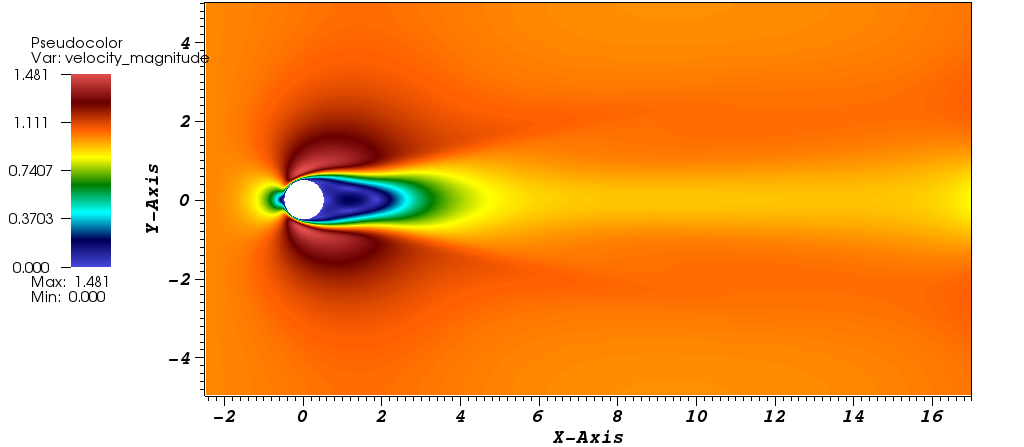
\includegraphics[width=\textwidth]{cyl/fom_avg}
         \caption{FOM}
         \label{fig:2_a}
     \end{subfigure}
     \hfill
     \begin{subfigure}[b]{0.3\textwidth}
         \centering
         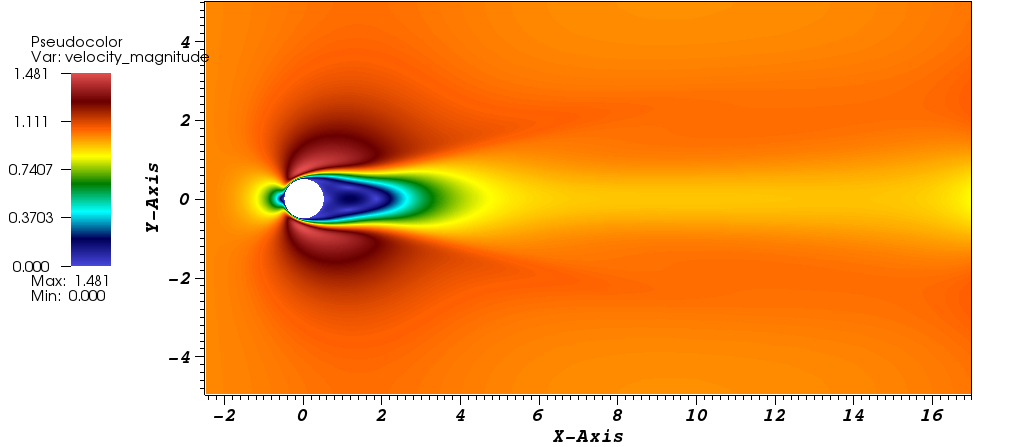
\includegraphics[width=\textwidth]{cyl/rom_avg}
         \caption{ROM with $N=20$}
         \label{fig:2_b}
     \end{subfigure}
     \hfill
     \begin{subfigure}[b]{0.3\textwidth}
         \centering
         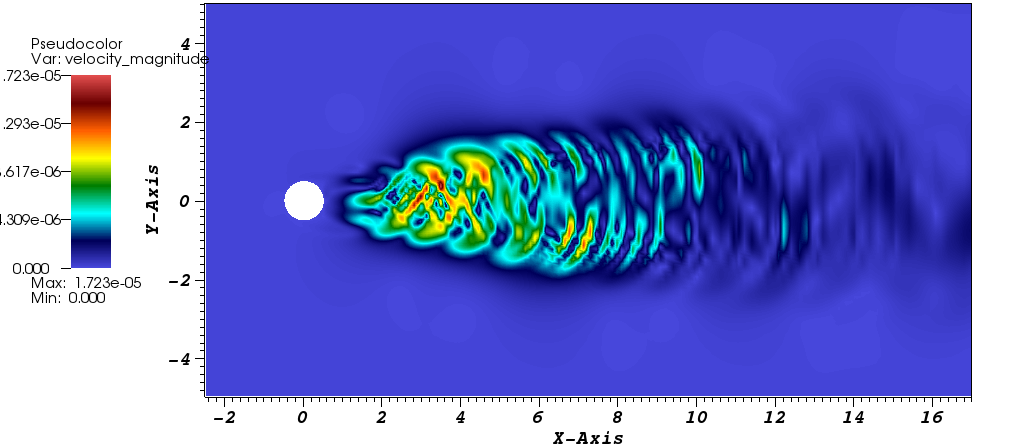
\includegraphics[width=\textwidth]{cyl/err_avg}
         \caption{Point-wise difference}
         \label{fig:2_c}
     \end{subfigure} 
     \caption{Reconstruction results with ROM with $N=20$ at $\rm Re=100$.
     \subref{fig:2_a}--\subref{fig:2_b}: Magnutide of averaged velocity of FOM
and ROM .  \subref{fig:2_c}: Point-wise difference between FOM and ROM with
maximum difference $\approx 1.5e-5$.}
     \label{fig:2}
\end{figure}

\subsection{Kovasznay Solution}

\noindent
Kovasznay \cite{kov48} gives an analytical solution to the steady-state
Navier-Stokes equations that is similar to the two-dimensional flow-field
behind a periodic array of cylinders,
\begin{align}
   u_x = 1-e^{\lambda x} \cos(2 \pi y), \quad u_y = \frac{\lambda}{2\pi}
   e^{\lambda x} \sin(2 \pi y),
\end{align}
where $\lambda \coloneqq \rm Re/2 - \sqrt{\rm Re^2/4 + 4\pi^2}$. 

The ROM reproduction results at $\rm Re=40$ are shown in Figure \ref{fig:3}.
\begin{figure}[!h]
     \centering
     \begin{subfigure}[b]{0.3\textwidth}
         \centering
         \includegraphics[width=\textwidth]{kov/fom}
         \caption{FOM}
         \label{fig:3_a}
     \end{subfigure}
     \begin{subfigure}[b]{0.3\textwidth}
         \centering
         \includegraphics[width=\textwidth]{kov/rom}
         \caption{ROM}
         \label{fig:3_b}
     \end{subfigure}
     \begin{subfigure}[b]{0.3\textwidth}
         \centering
         \includegraphics[width=\textwidth]{kov/err}
         \caption{Point-wise difference}
         \label{fig:3_c}
     \end{subfigure}
     \caption{ROM reproduction results for the Kovasznay flow \cite{kov48} 
at $\rm Re=40$.} \label{fig:3}
\end{figure}

\subsection{Convection in 2D Annulus}

\noindent
We consider a natural convection between the two concentric cylinders as
considered by Grigull \& Hauf \cite{grigull66} and presented by Van Dyke
\cite{vandyke82}. The inner cylinder (diameter $D$) is slightly heated with
with respect to the outer one (diameter $3D$). The Boussinesq approximation is
used to formulate the equations of motion, valid in situations where density
differences are small enough to be neglected everywhere except in the
gravitational forcing.  Normalizing the Navier-Stokes and energy equations with
$D$ for the length scale and $D/U$ for the time scale ($U \approx \sqrt{\alpha
g D (T_1-T_0)}$) is the characteristic velocity in the given problem), and
introducing nondimensional temperature $\theta=(T-T_0)/(T_1-T_0)$, where $T_0$
and $T_1$ are the respective temperatures of the outer and inner cylinders, the
governing equations take the nondimensional form
\begin{align}
   \pp{\bu}{t} + \bu \cdot \nabla \bu & = -\nabla p + \frac{1}{\sqrt{Gr}}
\nabla^2 \bu + \theta, \quad \nabla \bu = 0, \\ \pp{\theta}{t} + \bu \cdot
\nabla \theta & = \frac{1}{\sqrt{Gr}Pr} \nabla^2 \theta.
\end{align}
Here $\bu$ is the velocity vector, $p$ is the pressure, $\theta$ is the
temperature.  The Grashof and Prandtl numbers are defined as
\begin{equation}
   {\rm Gr} = \frac{\alpha g (T_1-T_0) D^3}{\nu^2}, \quad {\rm Pr} =
\frac{\nu}{\alpha},
\end{equation}
where $\nu$ is the kinematic viscosity, $\alpha$ is the volumetric thermal
expansion coefficient, and $g$ is the acceleration due to gravity. 

The ROM reproduction results at $\rm Gr=700000$ are shown in Figure
\ref{fig:4}.
The pMOR results with one to three anchor points are shown in Figure

\begin{figure}[!h]
     \centering
     \begin{subfigure}[b]{0.3\textwidth}
         \centering
         \includegraphics[width=\textwidth]{ann/fom}
         \caption{FOM}
         \label{fig:4_a}
     \end{subfigure}
     \begin{subfigure}[b]{0.3\textwidth}
         \centering
         \includegraphics[width=\textwidth]{ann/rom}
         \caption{ROM}
         \label{fig:4_b}
     \end{subfigure}
     \begin{subfigure}[b]{0.3\textwidth}
         \centering
         \includegraphics[width=\textwidth]{ann/err}
         \caption{Point-wise difference}
         \label{fig:4_c}
     \end{subfigure}
     \caption{ROM reproduction results for the annulus flow at $\rm
Gr=700000$.} \label{fig:4}
\end{figure}

\ref{fig:5}.  \begin{figure}[h]
     \centering
     \begin{subfigure}[b]{0.45\textwidth}
         \centering
         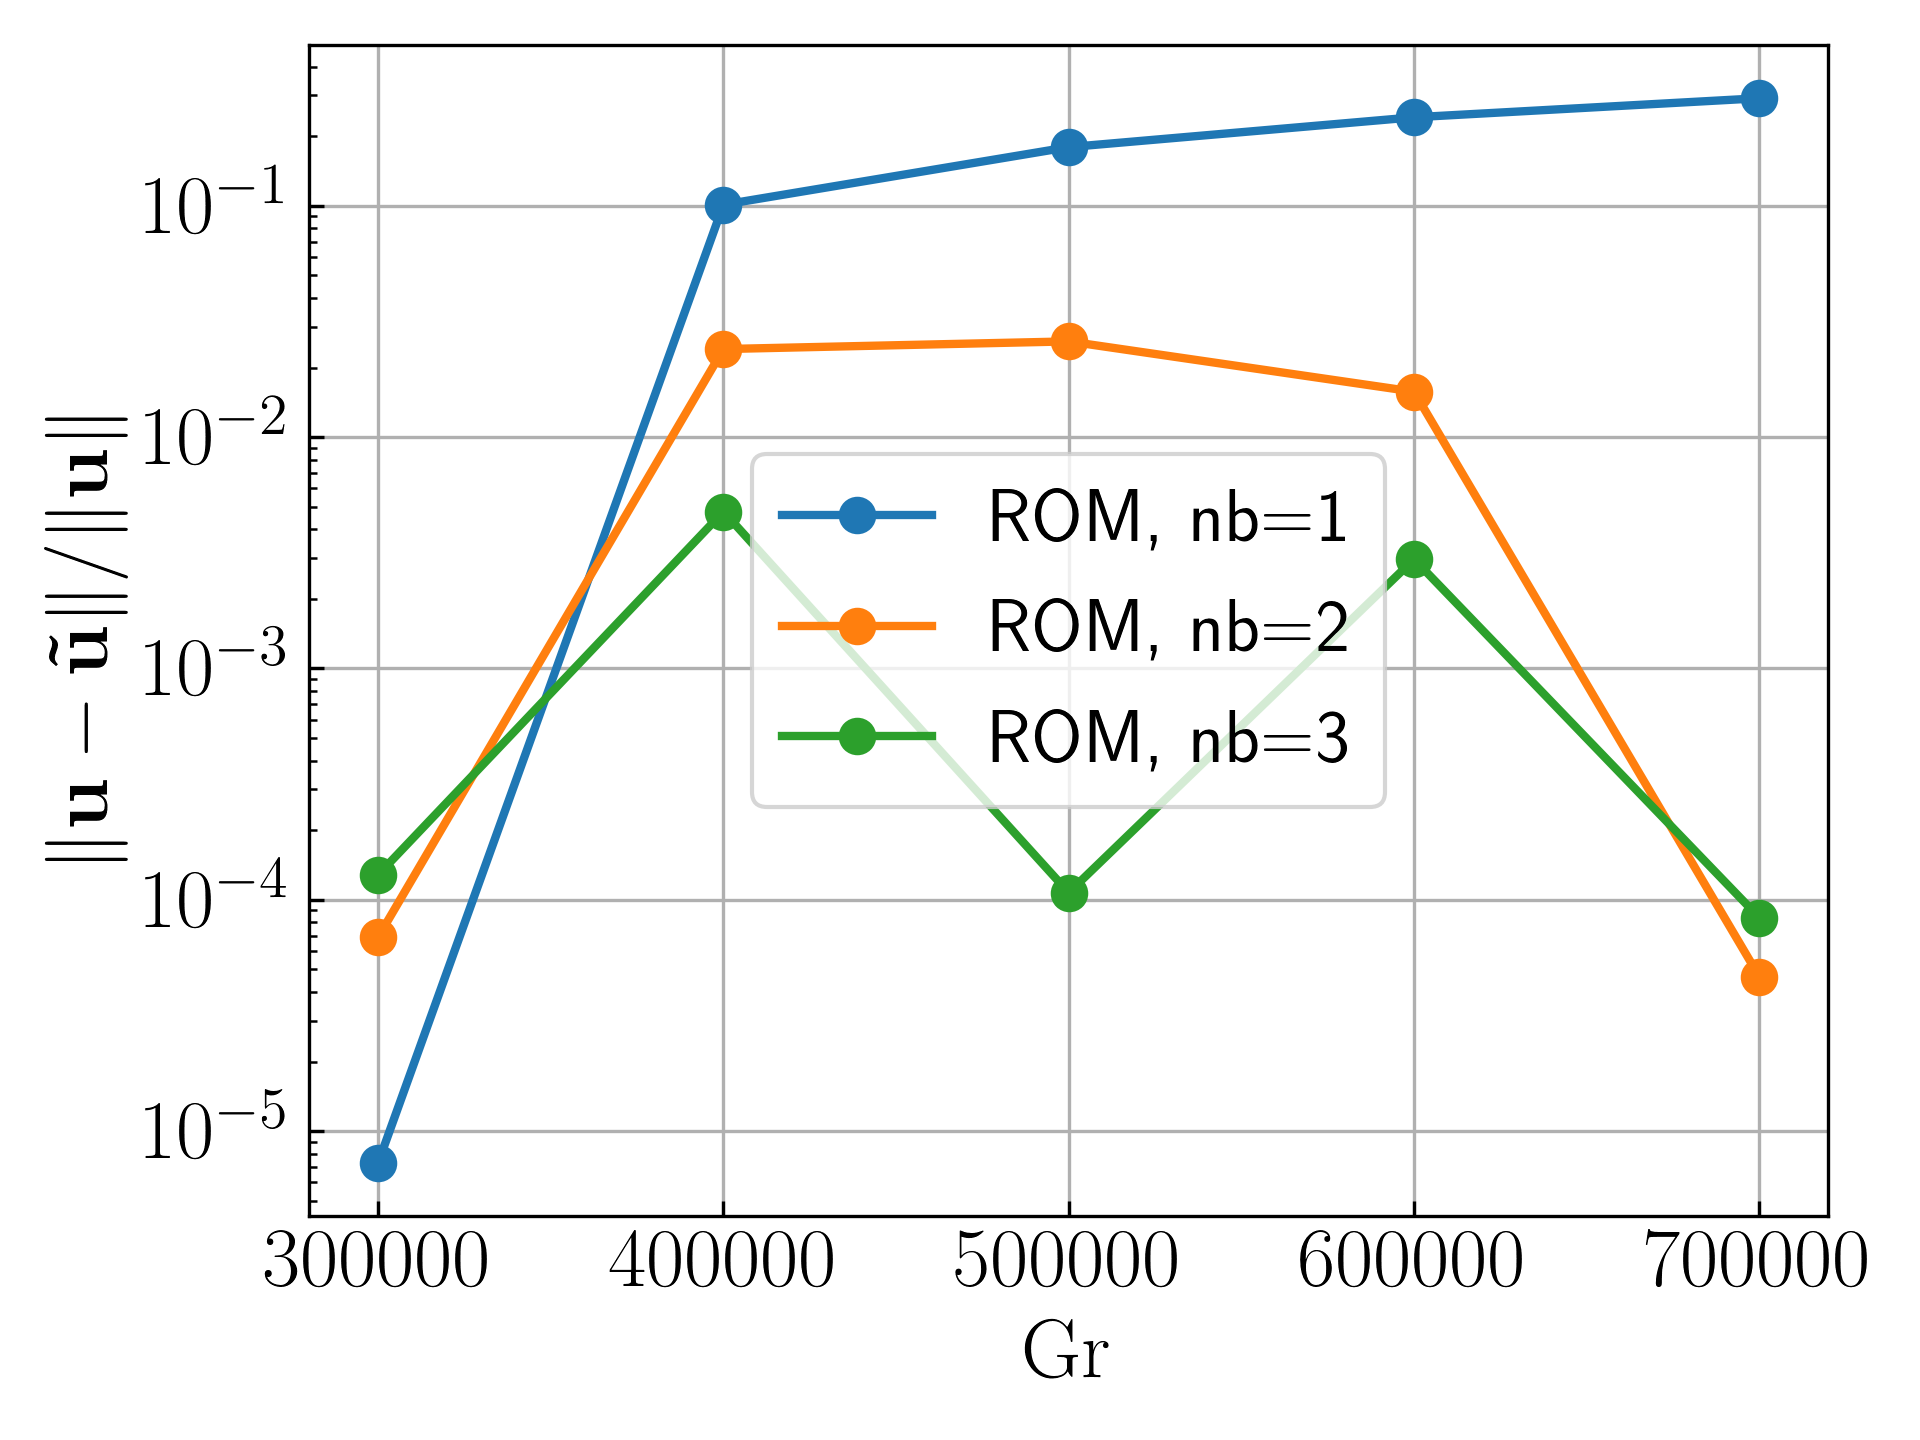
\includegraphics[width=\textwidth]{ann/err_gr}
         \caption{}
         \label{fig:3_a}
     \end{subfigure}
     \hfill
     \begin{subfigure}[b]{0.45\textwidth}
         \centering
         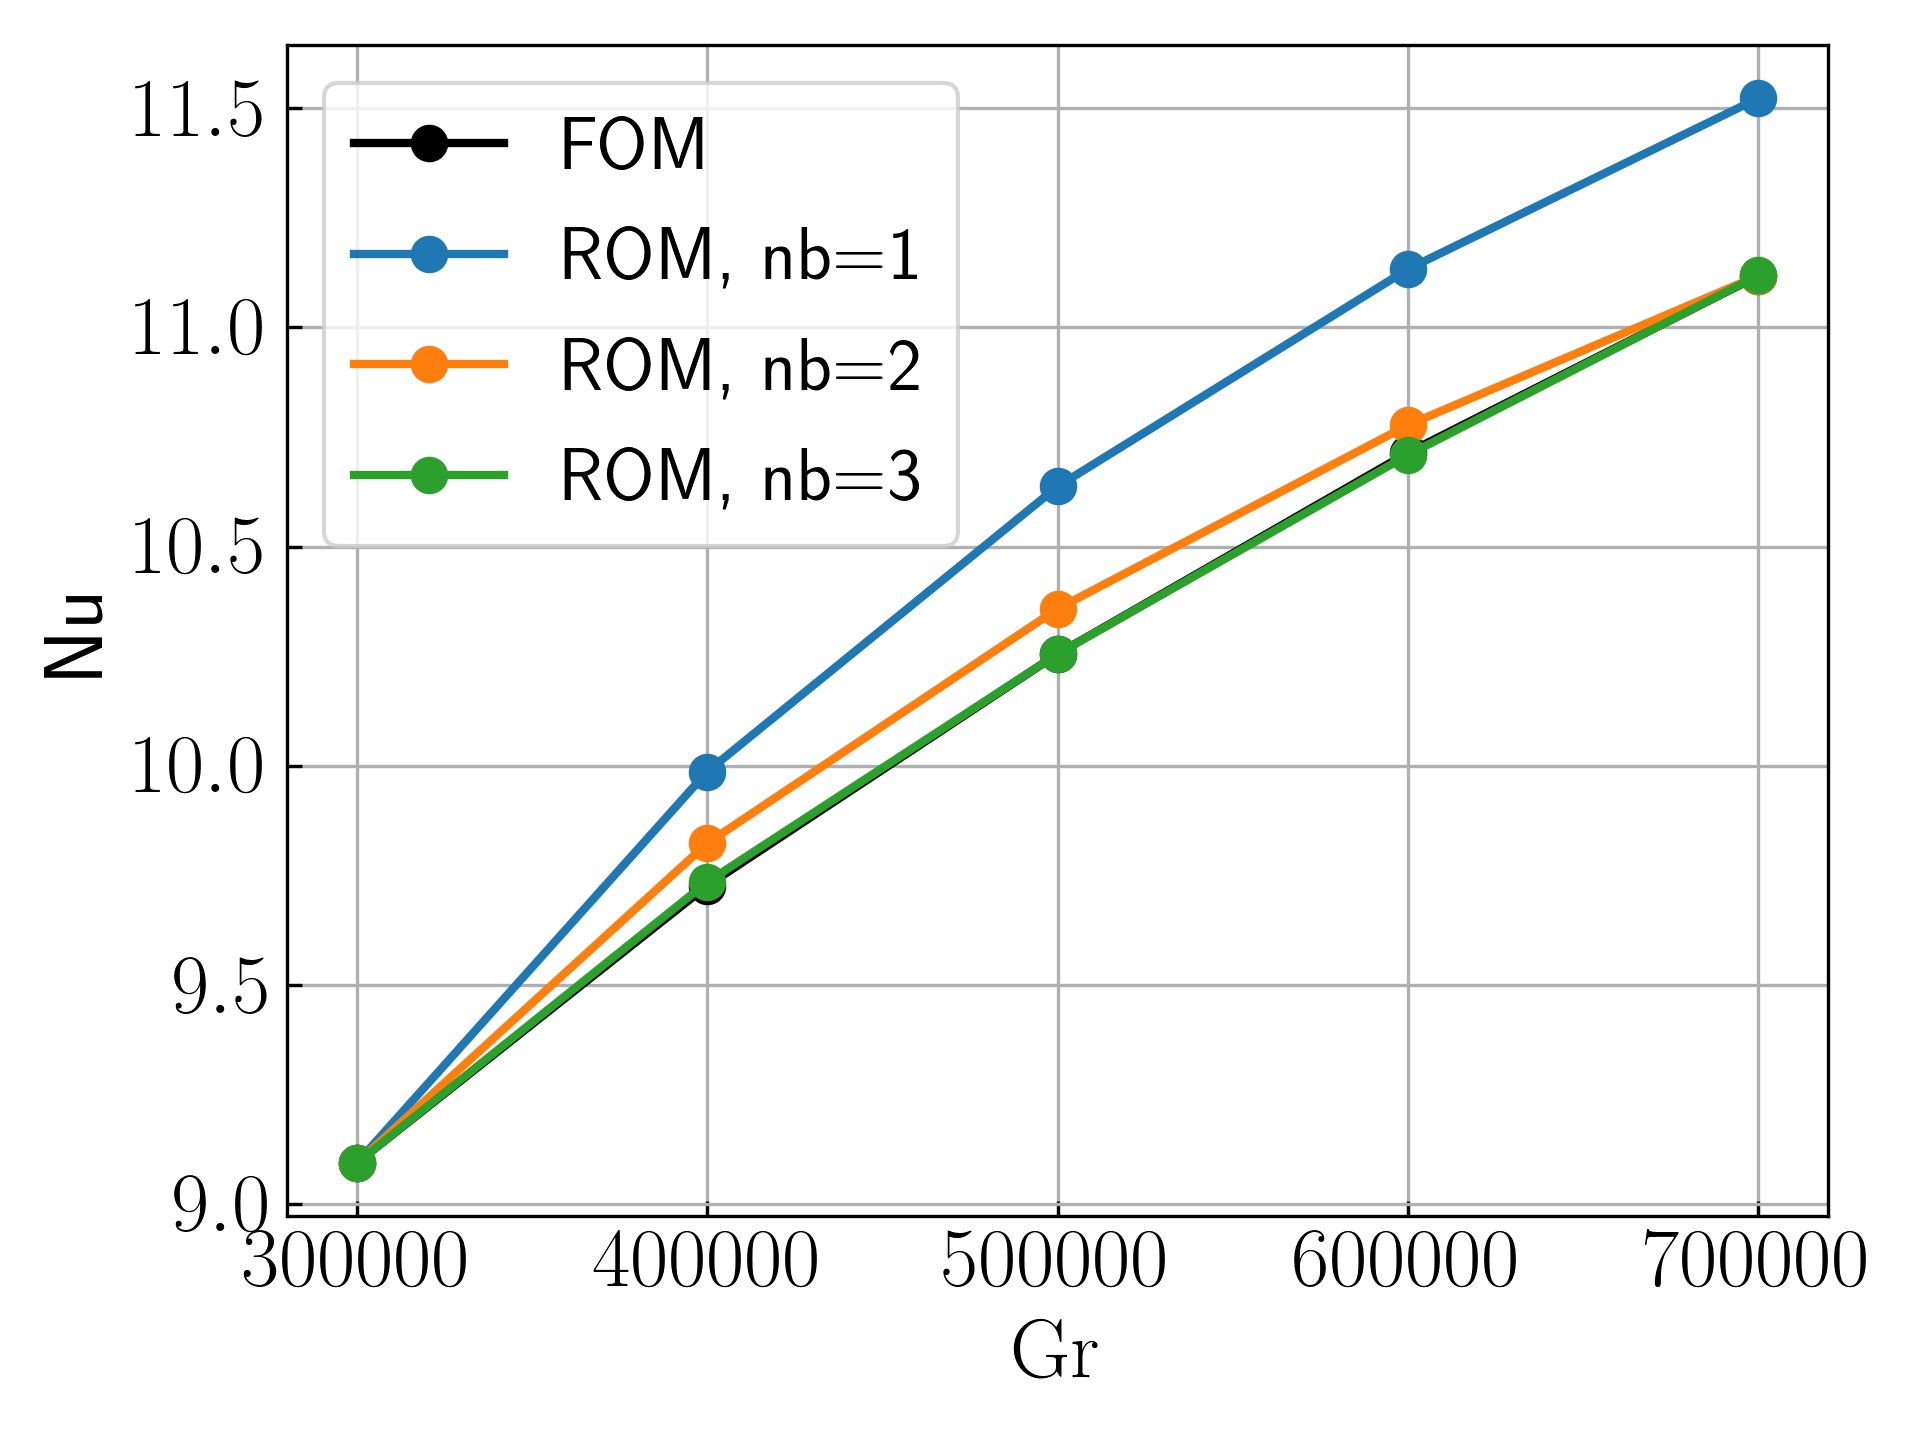
\includegraphics[width=\textwidth]{ann/nu_gr}
         \caption{}
         \label{fig:3_b}
     \end{subfigure}
     \caption{\subref{fig:3_a}: Relative $H^1$ error in the predicted solution
     with $N=1,~2,~3$.  \subref{fig:3_b}: Relative error in the predicted Nu
     with $N=1,~2,~3$; the ROM prediction values with $N=3$ are overlapped with
     the FOM values.} \label{fig:5}
\end{figure}

\subsection{Orr-Sommerfeld Problem}
We consider the evolution of small amplitude disturbances in channel flow \cite{rai1991direct,malik1985spectral}.
In this study the disturbance is taken to be an eigensolution of the
Orr-Sommerfeld equation. The advantage of using this problem as a test case is
that it has known solutions from linear theory.  The geometry consists of two
walls separated by a distance $2h$ with periodic boundary conditions in the
streamwise direction at $x = 0$ and $x = 2\pi$. The initial condition is
\begin{align}
   u^0(x,y) &= 1-(\frac{y}{h})^2 + \epsilon \hat{u} \\ 
   v^0(x,y) &= \epsilon \hat{v},
\end{align}
where $(\hat{u}, \hat{v})$ corresponds to the only unstable eigensolution (wave number unity) of the
Orr-Sommerfeld equation. The Reynolds number is $Re = U_c h / \nu =  7500$, based upon the
centerline velocity, $U_c = 1$. A constant body force is applied to sustain the mean flow.
The perturbation velocity is normalized to $|\hat{u}| = 1$ and $\epsilon$ is set to $.00001$.

According to the linear theory, the energy of the perturbation:
\begin{equation}
   E(t) = \int^{2\pi}_0 \int^1_{-1} \{ (1-y^2-u)^2 + v^2 \} ~dy~dx
\end{equation}
should grow as $e^{2\omega_i t}$, where $\omega_i = .002234976$. Following \cite{malik1985spectral},
we take as a measure of error the quantity: $error(t) = e^{2\omega_i t} - E(t_i)/E(0)$, where $E(t)$ is derived from 
the FOM and ROM solution at time $t=200$. In addition, we compute the error
in the growth rate at time $t = 200$ according to
\begin{equation}
   error_g = \frac{1}{\omega_i} \left|\omega_i - \frac{1}{2\Delta t}\ln \left(\frac{E(200)}{E(200-\Delta t)}\right) \right|
\end{equation}

Table \ref{table:1} shows the $error$ and $error_g$ for both FOM and ROM at $t=200$. The error in the growth rate is pretty good comparing to the result in FOM.

\begin{table}[h]
\caption{$error$ and $error_g$ for both FOM and ROM at $t=200$.}
\resizebox{\columnwidth}{!}{%
\begin{tabular}{|c|l|l|l|l|l|}
\hline
   \multicolumn{1}{|r|}{} & $t$ &  $\frac{E(t)}{E(0)}$    & $e^{(2 \omega_i t)}$ & $e^{(2 \omega_i t)}-\frac{E(t)}{E(0)}$ & \begin{tabular}[c]{@{}l@{}} $error_g$ \end{tabular} \\ \hline
FOM                    & 200  &  2.44363736 & 2.44486586       & -1.22850700E-03                & 5.77317855E-04                                                     \\ \hline
ROM                    & 200  &  2.45284455 & 2.44486586       & 7.97868317E-03                 & 3.64447902E-03                                                     \\ \hline
\end{tabular}
}
\label{table:1}
\end{table}
